Demuestra que el volumen de la región obtenida 
por rotar la región debajo de la gráfica de la parábola
$y=-x^2+2x+3$, $-1\leq x\leq 3$, al rededor del eje
$x$ es $512 \frac{\pi}{15}$. 
Véase la figura
\begin{figure}[H]
    \begin{center}
        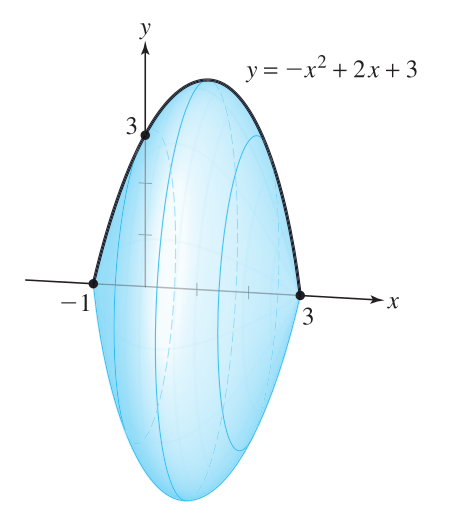
\includegraphics[width=0.3\textwidth]{img/Ej2/ej8b.png}
    \end{center}
\end{figure}
\begin{solution}
    Las secciones de corte con planos paralelos al plano \( yz \) son círculos de 
    radio \( y \), con área \( \pi y^2(x) = \pi (-x^2+2x+ 3)^2 \). Por el principio de 
    Cavalieri, el volumen de la región es 
    \begin{align*}
        \int_{-1}^3
        \pi y^2(x)
        \, dx
        &=
        \pi
        \int_{-1}^3
        (-x^2+2x+3)^2
        \, dx\\
        &=
        \pi
        \int_{-1}^3
        x^4-4x^3-2x^2+12x+9
        \,dx\\
        &=
        \left.
        \pi
        \left[ \frac{x^5}{5} -x^4- \frac{2x^3}{3} +6x^2+9x \right] \right|_{-1}^3\\
        &=
        \frac{512}{15} \pi
    \end{align*}
\end{solution}
